% Created by tikzDevice version 0.6.2-92-0ad2792 on 2013-03-30 14:47:46
% !TEX encoding = UTF-8 Unicode
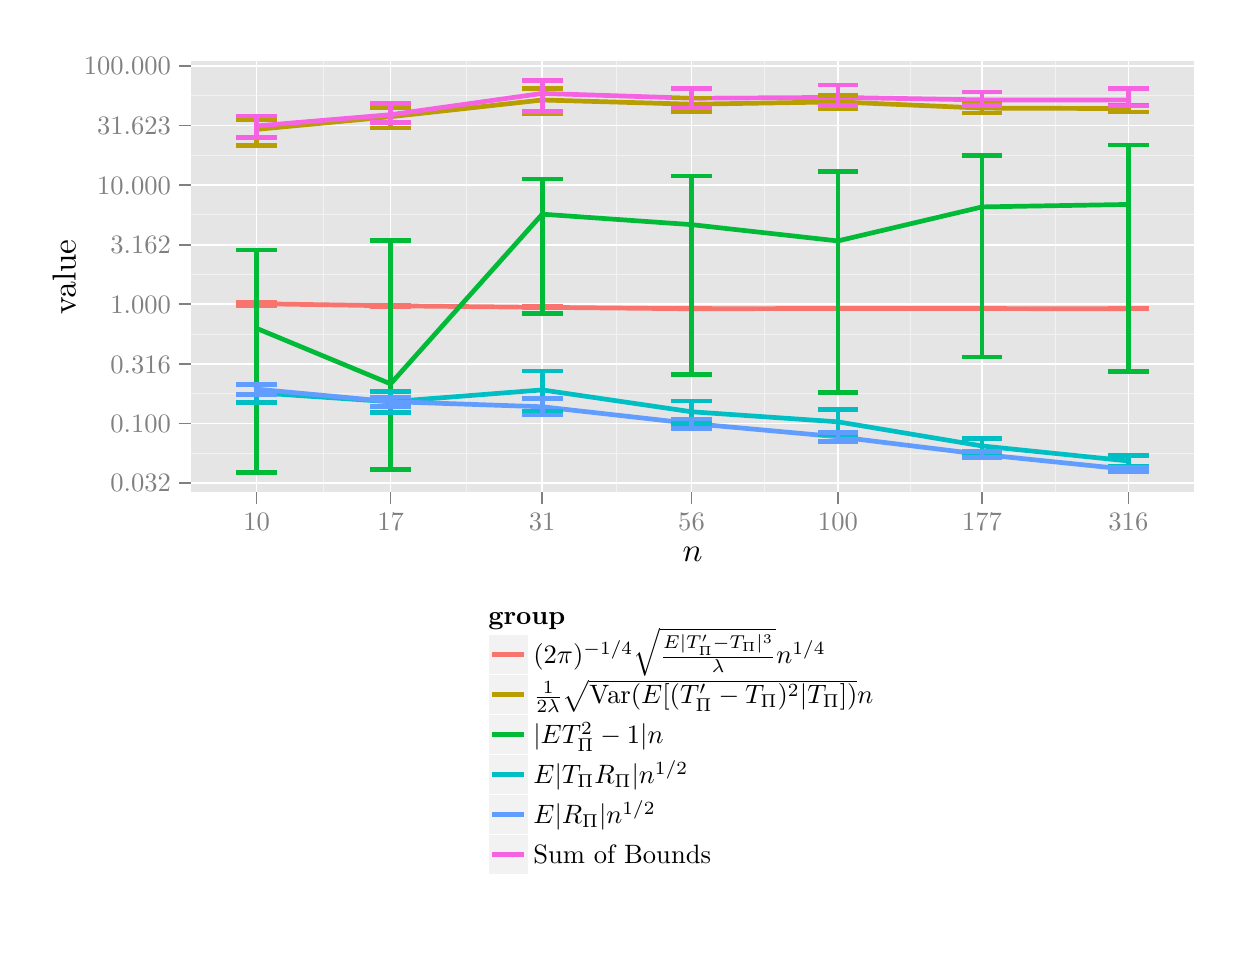
\begin{tikzpicture}[x=1pt,y=1pt]
\definecolor[named]{fillColor}{rgb}{1.00,1.00,1.00}
\path[use as bounding box,fill=fillColor,fill opacity=0.00] (0,0) rectangle (433.62,325.21);
\begin{scope}
\path[clip] (  0.00,  0.00) rectangle (433.62,325.21);
\definecolor[named]{drawColor}{rgb}{1.00,1.00,1.00}
\definecolor[named]{fillColor}{rgb}{1.00,1.00,1.00}

\path[draw=drawColor,line width= 0.6pt,line join=round,line cap=round,fill=fillColor] (  0.00,  0.00) rectangle (433.62,325.21);
\end{scope}
\begin{scope}
\path[clip] ( 58.88,157.27) rectangle (421.57,313.17);
\definecolor[named]{fillColor}{rgb}{0.90,0.90,0.90}

\path[fill=fillColor] ( 58.88,157.27) rectangle (421.57,313.17);
\definecolor[named]{drawColor}{rgb}{0.95,0.95,0.95}

\path[draw=drawColor,line width= 0.3pt,line join=round] ( 58.88,171.46) --
	(421.57,171.46);

\path[draw=drawColor,line width= 0.3pt,line join=round] ( 58.88,192.90) --
	(421.57,192.90);

\path[draw=drawColor,line width= 0.3pt,line join=round] ( 58.88,214.45) --
	(421.57,214.45);

\path[draw=drawColor,line width= 0.3pt,line join=round] ( 58.88,236.01) --
	(421.57,236.01);

\path[draw=drawColor,line width= 0.3pt,line join=round] ( 58.88,257.57) --
	(421.57,257.57);

\path[draw=drawColor,line width= 0.3pt,line join=round] ( 58.88,279.13) --
	(421.57,279.13);

\path[draw=drawColor,line width= 0.3pt,line join=round] ( 58.88,300.68) --
	(421.57,300.68);

\path[draw=drawColor,line width= 0.3pt,line join=round] (106.92,157.27) --
	(106.92,313.17);

\path[draw=drawColor,line width= 0.3pt,line join=round] (158.53,157.27) --
	(158.53,313.17);

\path[draw=drawColor,line width= 0.3pt,line join=round] (212.91,157.27) --
	(212.91,313.17);

\path[draw=drawColor,line width= 0.3pt,line join=round] (266.33,157.27) --
	(266.33,313.17);

\path[draw=drawColor,line width= 0.3pt,line join=round] (318.82,157.27) --
	(318.82,313.17);

\path[draw=drawColor,line width= 0.3pt,line join=round] (371.30,157.27) --
	(371.30,313.17);
\definecolor[named]{drawColor}{rgb}{1.00,1.00,1.00}

\path[draw=drawColor,line width= 0.6pt,line join=round] ( 58.88,160.79) --
	(421.57,160.79);

\path[draw=drawColor,line width= 0.6pt,line join=round] ( 58.88,182.12) --
	(421.57,182.12);

\path[draw=drawColor,line width= 0.6pt,line join=round] ( 58.88,203.67) --
	(421.57,203.67);

\path[draw=drawColor,line width= 0.6pt,line join=round] ( 58.88,225.24) --
	(421.57,225.24);

\path[draw=drawColor,line width= 0.6pt,line join=round] ( 58.88,246.79) --
	(421.57,246.79);

\path[draw=drawColor,line width= 0.6pt,line join=round] ( 58.88,268.35) --
	(421.57,268.35);

\path[draw=drawColor,line width= 0.6pt,line join=round] ( 58.88,289.90) --
	(421.57,289.90);

\path[draw=drawColor,line width= 0.6pt,line join=round] ( 58.88,311.46) --
	(421.57,311.46);

\path[draw=drawColor,line width= 0.6pt,line join=round] ( 82.72,157.27) --
	( 82.72,313.17);

\path[draw=drawColor,line width= 0.6pt,line join=round] (131.13,157.27) --
	(131.13,313.17);

\path[draw=drawColor,line width= 0.6pt,line join=round] (185.93,157.27) --
	(185.93,313.17);

\path[draw=drawColor,line width= 0.6pt,line join=round] (239.88,157.27) --
	(239.88,313.17);

\path[draw=drawColor,line width= 0.6pt,line join=round] (292.78,157.27) --
	(292.78,313.17);

\path[draw=drawColor,line width= 0.6pt,line join=round] (344.86,157.27) --
	(344.86,313.17);

\path[draw=drawColor,line width= 0.6pt,line join=round] (397.74,157.27) --
	(397.74,313.17);
\definecolor[named]{drawColor}{rgb}{0.97,0.46,0.43}

\path[draw=drawColor,line width= 1.7pt,line join=round] ( 82.72,225.46) --
	(131.13,224.70) --
	(185.93,224.15) --
	(239.88,223.63) --
	(292.78,223.74) --
	(344.86,223.71) --
	(397.74,223.61);
\definecolor[named]{drawColor}{rgb}{0.72,0.62,0.00}

\path[draw=drawColor,line width= 1.7pt,line join=round] ( 82.72,288.45) --
	(131.13,293.03) --
	(185.93,299.07) --
	(239.88,297.55) --
	(292.78,298.39) --
	(344.86,296.14) --
	(397.74,295.98);
\definecolor[named]{drawColor}{rgb}{0.00,0.73,0.22}

\path[draw=drawColor,line width= 1.7pt,line join=round] ( 82.72,216.56) --
	(131.13,196.50) --
	(185.93,257.81) --
	(239.88,254.03) --
	(292.78,248.15) --
	(344.86,260.44) --
	(397.74,261.33);
\definecolor[named]{drawColor}{rgb}{0.00,0.75,0.77}

\path[draw=drawColor,line width= 1.7pt,line join=round] ( 82.72,193.30) --
	(131.13,190.04) --
	(185.93,194.31) --
	(239.88,186.41) --
	(292.78,182.78) --
	(344.86,174.06) --
	(397.74,168.64);
\definecolor[named]{drawColor}{rgb}{0.38,0.61,1.00}

\path[draw=drawColor,line width= 1.7pt,line join=round] ( 82.72,194.58) --
	(131.13,190.08) --
	(185.93,188.22) --
	(239.88,182.17) --
	(292.78,177.38) --
	(344.86,170.99) --
	(397.74,165.58);
\definecolor[named]{drawColor}{rgb}{0.96,0.39,0.89}

\path[draw=drawColor,line width= 1.7pt,line join=round] ( 82.72,289.70) --
	(131.13,293.76) --
	(185.93,301.45) --
	(239.88,299.71) --
	(292.78,300.01) --
	(344.86,299.11) --
	(397.74,299.08);
\definecolor[named]{drawColor}{rgb}{0.97,0.46,0.43}

\path[draw=drawColor,line width= 1.7pt,line join=round] ( 75.37,226.01) --
	( 90.07,226.01);

\path[draw=drawColor,line width= 1.7pt,line join=round] ( 82.72,226.01) --
	( 82.72,224.89);

\path[draw=drawColor,line width= 1.7pt,line join=round] ( 75.37,224.89) --
	( 90.07,224.89);

\path[draw=drawColor,line width= 1.7pt,line join=round] (123.78,225.03) --
	(138.48,225.03);

\path[draw=drawColor,line width= 1.7pt,line join=round] (131.13,225.03) --
	(131.13,224.39);

\path[draw=drawColor,line width= 1.7pt,line join=round] (123.78,224.39) --
	(138.48,224.39);

\path[draw=drawColor,line width= 1.7pt,line join=round] (178.58,224.34) --
	(193.28,224.34);

\path[draw=drawColor,line width= 1.7pt,line join=round] (185.93,224.34) --
	(185.93,223.99);

\path[draw=drawColor,line width= 1.7pt,line join=round] (178.58,223.99) --
	(193.28,223.99);

\path[draw=drawColor,line width= 1.7pt,line join=round] (232.53,223.69) --
	(247.23,223.69);

\path[draw=drawColor,line width= 1.7pt,line join=round] (239.88,223.69) --
	(239.88,223.56);

\path[draw=drawColor,line width= 1.7pt,line join=round] (232.53,223.56) --
	(247.23,223.56);

\path[draw=drawColor,line width= 1.7pt,line join=round] (285.42,223.77) --
	(300.13,223.77);

\path[draw=drawColor,line width= 1.7pt,line join=round] (292.78,223.77) --
	(292.78,223.71);

\path[draw=drawColor,line width= 1.7pt,line join=round] (285.42,223.71) --
	(300.13,223.71);

\path[draw=drawColor,line width= 1.7pt,line join=round] (337.51,223.72) --
	(352.22,223.72);

\path[draw=drawColor,line width= 1.7pt,line join=round] (344.86,223.72) --
	(344.86,223.70);

\path[draw=drawColor,line width= 1.7pt,line join=round] (337.51,223.70) --
	(352.22,223.70);

\path[draw=drawColor,line width= 1.7pt,line join=round] (390.39,223.61) --
	(405.09,223.61);

\path[draw=drawColor,line width= 1.7pt,line join=round] (397.74,223.61) --
	(397.74,223.61);

\path[draw=drawColor,line width= 1.7pt,line join=round] (390.39,223.61) --
	(405.09,223.61);
\definecolor[named]{drawColor}{rgb}{0.72,0.62,0.00}

\path[draw=drawColor,line width= 1.7pt,line join=round] ( 75.37,291.92) --
	( 90.07,291.92);

\path[draw=drawColor,line width= 1.7pt,line join=round] ( 82.72,291.92) --
	( 82.72,282.60);

\path[draw=drawColor,line width= 1.7pt,line join=round] ( 75.37,282.60) --
	( 90.07,282.60);

\path[draw=drawColor,line width= 1.7pt,line join=round] (123.78,296.38) --
	(138.48,296.38);

\path[draw=drawColor,line width= 1.7pt,line join=round] (131.13,296.38) --
	(131.13,288.94);

\path[draw=drawColor,line width= 1.7pt,line join=round] (123.78,288.94) --
	(138.48,288.94);

\path[draw=drawColor,line width= 1.7pt,line join=round] (178.58,303.20) --
	(193.28,303.20);

\path[draw=drawColor,line width= 1.7pt,line join=round] (185.93,303.20) --
	(185.93,294.04);

\path[draw=drawColor,line width= 1.7pt,line join=round] (178.58,294.04) --
	(193.28,294.04);

\path[draw=drawColor,line width= 1.7pt,line join=round] (232.53,299.75) --
	(247.23,299.75);

\path[draw=drawColor,line width= 1.7pt,line join=round] (239.88,299.75) --
	(239.88,294.91);

\path[draw=drawColor,line width= 1.7pt,line join=round] (232.53,294.91) --
	(247.23,294.91);

\path[draw=drawColor,line width= 1.7pt,line join=round] (285.42,300.72) --
	(300.13,300.72);

\path[draw=drawColor,line width= 1.7pt,line join=round] (292.78,300.72) --
	(292.78,295.84);

\path[draw=drawColor,line width= 1.7pt,line join=round] (285.42,295.84) --
	(300.13,295.84);

\path[draw=drawColor,line width= 1.7pt,line join=round] (337.51,297.73) --
	(352.22,297.73);

\path[draw=drawColor,line width= 1.7pt,line join=round] (344.86,297.73) --
	(344.86,294.36);

\path[draw=drawColor,line width= 1.7pt,line join=round] (337.51,294.36) --
	(352.22,294.36);

\path[draw=drawColor,line width= 1.7pt,line join=round] (390.39,297.03) --
	(405.09,297.03);

\path[draw=drawColor,line width= 1.7pt,line join=round] (397.74,297.03) --
	(397.74,294.78);

\path[draw=drawColor,line width= 1.7pt,line join=round] (390.39,294.78) --
	(405.09,294.78);
\definecolor[named]{drawColor}{rgb}{0.00,0.73,0.22}

\path[draw=drawColor,line width= 1.7pt,line join=round] ( 75.37,244.85) --
	( 90.07,244.85);

\path[draw=drawColor,line width= 1.7pt,line join=round] ( 82.72,244.85) --
	( 82.72,164.35);

\path[draw=drawColor,line width= 1.7pt,line join=round] ( 75.37,164.35) --
	( 90.07,164.35);

\path[draw=drawColor,line width= 1.7pt,line join=round] (123.78,248.34) --
	(138.48,248.34);

\path[draw=drawColor,line width= 1.7pt,line join=round] (131.13,248.34) --
	(131.13,165.54);

\path[draw=drawColor,line width= 1.7pt,line join=round] (123.78,165.54) --
	(138.48,165.54);

\path[draw=drawColor,line width= 1.7pt,line join=round] (178.58,270.49) --
	(193.28,270.49);

\path[draw=drawColor,line width= 1.7pt,line join=round] (185.93,270.49) --
	(185.93,221.84);

\path[draw=drawColor,line width= 1.7pt,line join=round] (178.58,221.84) --
	(193.28,221.84);

\path[draw=drawColor,line width= 1.7pt,line join=round] (232.53,271.56) --
	(247.23,271.56);

\path[draw=drawColor,line width= 1.7pt,line join=round] (239.88,271.56) --
	(239.88,199.80);

\path[draw=drawColor,line width= 1.7pt,line join=round] (232.53,199.80) --
	(247.23,199.80);

\path[draw=drawColor,line width= 1.7pt,line join=round] (285.42,273.25) --
	(300.13,273.25);

\path[draw=drawColor,line width= 1.7pt,line join=round] (292.78,273.25) --
	(292.78,193.31);

\path[draw=drawColor,line width= 1.7pt,line join=round] (285.42,193.31) --
	(300.13,193.31);

\path[draw=drawColor,line width= 1.7pt,line join=round] (337.51,279.11) --
	(352.22,279.11);

\path[draw=drawColor,line width= 1.7pt,line join=round] (344.86,279.11) --
	(344.86,206.20);

\path[draw=drawColor,line width= 1.7pt,line join=round] (337.51,206.20) --
	(352.22,206.20);

\path[draw=drawColor,line width= 1.7pt,line join=round] (390.39,282.83) --
	(405.09,282.83);

\path[draw=drawColor,line width= 1.7pt,line join=round] (397.74,282.83) --
	(397.74,200.96);

\path[draw=drawColor,line width= 1.7pt,line join=round] (390.39,200.96) --
	(405.09,200.96);
\definecolor[named]{drawColor}{rgb}{0.00,0.75,0.77}

\path[draw=drawColor,line width= 1.7pt,line join=round] ( 75.37,196.35) --
	( 90.07,196.35);

\path[draw=drawColor,line width= 1.7pt,line join=round] ( 82.72,196.35) --
	( 82.72,189.66);

\path[draw=drawColor,line width= 1.7pt,line join=round] ( 75.37,189.66) --
	( 90.07,189.66);

\path[draw=drawColor,line width= 1.7pt,line join=round] (123.78,193.71) --
	(138.48,193.71);

\path[draw=drawColor,line width= 1.7pt,line join=round] (131.13,193.71) --
	(131.13,186.21);

\path[draw=drawColor,line width= 1.7pt,line join=round] (123.78,186.21) --
	(138.48,186.21);

\path[draw=drawColor,line width= 1.7pt,line join=round] (178.58,201.10) --
	(193.28,201.10);

\path[draw=drawColor,line width= 1.7pt,line join=round] (185.93,201.10) --
	(185.93,186.74);

\path[draw=drawColor,line width= 1.7pt,line join=round] (178.58,186.74) --
	(193.28,186.74);

\path[draw=drawColor,line width= 1.7pt,line join=round] (232.53,190.27) --
	(247.23,190.27);

\path[draw=drawColor,line width= 1.7pt,line join=round] (239.88,190.27) --
	(239.88,182.24);

\path[draw=drawColor,line width= 1.7pt,line join=round] (232.53,182.24) --
	(247.23,182.24);

\path[draw=drawColor,line width= 1.7pt,line join=round] (285.42,187.19) --
	(300.13,187.19);

\path[draw=drawColor,line width= 1.7pt,line join=round] (292.78,187.19) --
	(292.78,178.04);

\path[draw=drawColor,line width= 1.7pt,line join=round] (285.42,178.04) --
	(300.13,178.04);

\path[draw=drawColor,line width= 1.7pt,line join=round] (337.51,176.74) --
	(352.22,176.74);

\path[draw=drawColor,line width= 1.7pt,line join=round] (344.86,176.74) --
	(344.86,171.36);

\path[draw=drawColor,line width= 1.7pt,line join=round] (337.51,171.36) --
	(352.22,171.36);

\path[draw=drawColor,line width= 1.7pt,line join=round] (390.39,170.50) --
	(405.09,170.50);

\path[draw=drawColor,line width= 1.7pt,line join=round] (397.74,170.50) --
	(397.74,166.86);

\path[draw=drawColor,line width= 1.7pt,line join=round] (390.39,166.86) --
	(405.09,166.86);
\definecolor[named]{drawColor}{rgb}{0.38,0.61,1.00}

\path[draw=drawColor,line width= 1.7pt,line join=round] ( 75.37,196.35) --
	( 90.07,196.35);

\path[draw=drawColor,line width= 1.7pt,line join=round] ( 82.72,196.35) --
	( 82.72,192.57);

\path[draw=drawColor,line width= 1.7pt,line join=round] ( 75.37,192.57) --
	( 90.07,192.57);

\path[draw=drawColor,line width= 1.7pt,line join=round] (123.78,191.73) --
	(138.48,191.73);

\path[draw=drawColor,line width= 1.7pt,line join=round] (131.13,191.73) --
	(131.13,188.38);

\path[draw=drawColor,line width= 1.7pt,line join=round] (123.78,188.38) --
	(138.48,188.38);

\path[draw=drawColor,line width= 1.7pt,line join=round] (178.58,191.29) --
	(193.28,191.29);

\path[draw=drawColor,line width= 1.7pt,line join=round] (185.93,191.29) --
	(185.93,185.23);

\path[draw=drawColor,line width= 1.7pt,line join=round] (178.58,185.23) --
	(193.28,185.23);

\path[draw=drawColor,line width= 1.7pt,line join=round] (232.53,183.79) --
	(247.23,183.79);

\path[draw=drawColor,line width= 1.7pt,line join=round] (239.88,183.79) --
	(239.88,180.30);

\path[draw=drawColor,line width= 1.7pt,line join=round] (232.53,180.30) --
	(247.23,180.30);

\path[draw=drawColor,line width= 1.7pt,line join=round] (285.42,179.04) --
	(300.13,179.04);

\path[draw=drawColor,line width= 1.7pt,line join=round] (292.78,179.04) --
	(292.78,175.66);

\path[draw=drawColor,line width= 1.7pt,line join=round] (285.42,175.66) --
	(300.13,175.66);

\path[draw=drawColor,line width= 1.7pt,line join=round] (337.51,172.13) --
	(352.22,172.13);

\path[draw=drawColor,line width= 1.7pt,line join=round] (344.86,172.13) --
	(344.86,170.00);

\path[draw=drawColor,line width= 1.7pt,line join=round] (337.51,170.00) --
	(352.22,170.00);

\path[draw=drawColor,line width= 1.7pt,line join=round] (390.39,166.27) --
	(405.09,166.27);

\path[draw=drawColor,line width= 1.7pt,line join=round] (397.74,166.27) --
	(397.74,164.80);

\path[draw=drawColor,line width= 1.7pt,line join=round] (390.39,164.80) --
	(405.09,164.80);
\definecolor[named]{drawColor}{rgb}{0.96,0.39,0.89}

\path[draw=drawColor,line width= 1.7pt,line join=round] ( 75.37,293.28) --
	( 90.07,293.28);

\path[draw=drawColor,line width= 1.7pt,line join=round] ( 82.72,293.28) --
	( 82.72,285.60);

\path[draw=drawColor,line width= 1.7pt,line join=round] ( 75.37,285.60) --
	( 90.07,285.60);

\path[draw=drawColor,line width= 1.7pt,line join=round] (123.78,297.70) --
	(138.48,297.70);

\path[draw=drawColor,line width= 1.7pt,line join=round] (131.13,297.70) --
	(131.13,290.92);

\path[draw=drawColor,line width= 1.7pt,line join=round] (123.78,290.92) --
	(138.48,290.92);

\path[draw=drawColor,line width= 1.7pt,line join=round] (178.58,306.08) --
	(193.28,306.08);

\path[draw=drawColor,line width= 1.7pt,line join=round] (185.93,306.08) --
	(185.93,294.93);

\path[draw=drawColor,line width= 1.7pt,line join=round] (178.58,294.93) --
	(193.28,294.93);

\path[draw=drawColor,line width= 1.7pt,line join=round] (232.53,303.31) --
	(247.23,303.31);

\path[draw=drawColor,line width= 1.7pt,line join=round] (239.88,303.31) --
	(239.88,296.23);

\path[draw=drawColor,line width= 1.7pt,line join=round] (232.53,296.23) --
	(247.23,296.23);

\path[draw=drawColor,line width= 1.7pt,line join=round] (285.42,304.54) --
	(300.13,304.54);

\path[draw=drawColor,line width= 1.7pt,line join=round] (292.78,304.54) --
	(292.78,297.13);

\path[draw=drawColor,line width= 1.7pt,line join=round] (285.42,297.13) --
	(300.13,297.13);

\path[draw=drawColor,line width= 1.7pt,line join=round] (337.51,301.98) --
	(352.22,301.98);

\path[draw=drawColor,line width= 1.7pt,line join=round] (344.86,301.98) --
	(344.86,297.03);

\path[draw=drawColor,line width= 1.7pt,line join=round] (337.51,297.03) --
	(352.22,297.03);

\path[draw=drawColor,line width= 1.7pt,line join=round] (390.39,303.19) --
	(405.09,303.19);

\path[draw=drawColor,line width= 1.7pt,line join=round] (397.74,303.19) --
	(397.74,296.89);

\path[draw=drawColor,line width= 1.7pt,line join=round] (390.39,296.89) --
	(405.09,296.89);
\end{scope}
\begin{scope}
\path[clip] (  0.00,  0.00) rectangle (433.62,325.21);
\definecolor[named]{drawColor}{rgb}{0.50,0.50,0.50}

\node[text=drawColor,anchor=base east,inner sep=0pt, outer sep=0pt, scale=  0.96] at ( 51.77,157.48) {0.032};

\node[text=drawColor,anchor=base east,inner sep=0pt, outer sep=0pt, scale=  0.96] at ( 51.77,178.82) {0.100};

\node[text=drawColor,anchor=base east,inner sep=0pt, outer sep=0pt, scale=  0.96] at ( 51.77,200.36) {0.316};

\node[text=drawColor,anchor=base east,inner sep=0pt, outer sep=0pt, scale=  0.96] at ( 51.77,221.93) {1.000};

\node[text=drawColor,anchor=base east,inner sep=0pt, outer sep=0pt, scale=  0.96] at ( 51.77,243.48) {3.162};

\node[text=drawColor,anchor=base east,inner sep=0pt, outer sep=0pt, scale=  0.96] at ( 51.77,265.04) {10.000};

\node[text=drawColor,anchor=base east,inner sep=0pt, outer sep=0pt, scale=  0.96] at ( 51.77,286.60) {31.623};

\node[text=drawColor,anchor=base east,inner sep=0pt, outer sep=0pt, scale=  0.96] at ( 51.77,308.15) {100.000};
\end{scope}
\begin{scope}
\path[clip] (  0.00,  0.00) rectangle (433.62,325.21);
\definecolor[named]{drawColor}{rgb}{0.50,0.50,0.50}

\path[draw=drawColor,line width= 0.6pt,line join=round] ( 54.61,160.79) --
	( 58.88,160.79);

\path[draw=drawColor,line width= 0.6pt,line join=round] ( 54.61,182.12) --
	( 58.88,182.12);

\path[draw=drawColor,line width= 0.6pt,line join=round] ( 54.61,203.67) --
	( 58.88,203.67);

\path[draw=drawColor,line width= 0.6pt,line join=round] ( 54.61,225.24) --
	( 58.88,225.24);

\path[draw=drawColor,line width= 0.6pt,line join=round] ( 54.61,246.79) --
	( 58.88,246.79);

\path[draw=drawColor,line width= 0.6pt,line join=round] ( 54.61,268.35) --
	( 58.88,268.35);

\path[draw=drawColor,line width= 0.6pt,line join=round] ( 54.61,289.90) --
	( 58.88,289.90);

\path[draw=drawColor,line width= 0.6pt,line join=round] ( 54.61,311.46) --
	( 58.88,311.46);
\end{scope}
\begin{scope}
\path[clip] (  0.00,  0.00) rectangle (433.62,325.21);
\definecolor[named]{drawColor}{rgb}{0.50,0.50,0.50}

\path[draw=drawColor,line width= 0.6pt,line join=round] ( 82.72,153.00) --
	( 82.72,157.27);

\path[draw=drawColor,line width= 0.6pt,line join=round] (131.13,153.00) --
	(131.13,157.27);

\path[draw=drawColor,line width= 0.6pt,line join=round] (185.93,153.00) --
	(185.93,157.27);

\path[draw=drawColor,line width= 0.6pt,line join=round] (239.88,153.00) --
	(239.88,157.27);

\path[draw=drawColor,line width= 0.6pt,line join=round] (292.78,153.00) --
	(292.78,157.27);

\path[draw=drawColor,line width= 0.6pt,line join=round] (344.86,153.00) --
	(344.86,157.27);

\path[draw=drawColor,line width= 0.6pt,line join=round] (397.74,153.00) --
	(397.74,157.27);
\end{scope}
\begin{scope}
\path[clip] (  0.00,  0.00) rectangle (433.62,325.21);
\definecolor[named]{drawColor}{rgb}{0.50,0.50,0.50}

\node[text=drawColor,anchor=base,inner sep=0pt, outer sep=0pt, scale=  0.96] at ( 82.72,143.54) {10};

\node[text=drawColor,anchor=base,inner sep=0pt, outer sep=0pt, scale=  0.96] at (131.13,143.54) {17};

\node[text=drawColor,anchor=base,inner sep=0pt, outer sep=0pt, scale=  0.96] at (185.93,143.54) {31};

\node[text=drawColor,anchor=base,inner sep=0pt, outer sep=0pt, scale=  0.96] at (239.88,143.54) {56};

\node[text=drawColor,anchor=base,inner sep=0pt, outer sep=0pt, scale=  0.96] at (292.78,143.54) {100};

\node[text=drawColor,anchor=base,inner sep=0pt, outer sep=0pt, scale=  0.96] at (344.86,143.54) {177};

\node[text=drawColor,anchor=base,inner sep=0pt, outer sep=0pt, scale=  0.96] at (397.74,143.54) {316};
\end{scope}
\begin{scope}
\path[clip] (  0.00,  0.00) rectangle (433.62,325.21);
\definecolor[named]{drawColor}{rgb}{0.00,0.00,0.00}

\node[text=drawColor,anchor=base,inner sep=0pt, outer sep=0pt, scale=  1.20] at (240.23,132.27) {$n$};
\end{scope}
\begin{scope}
\path[clip] (  0.00,  0.00) rectangle (433.62,325.21);
\definecolor[named]{drawColor}{rgb}{0.00,0.00,0.00}

\node[text=drawColor,rotate= 90.00,anchor=base,inner sep=0pt, outer sep=0pt, scale=  1.20] at ( 17.30,235.22) {value};
\end{scope}
\begin{scope}
\path[clip] (  0.00,  0.00) rectangle (433.62,325.21);
\definecolor[named]{fillColor}{rgb}{1.00,1.00,1.00}

\path[fill=fillColor] (162.21, 14.89) rectangle (318.25,120.39);
\end{scope}
\begin{scope}
\path[clip] (  0.00,  0.00) rectangle (433.62,325.21);
\definecolor[named]{drawColor}{rgb}{0.00,0.00,0.00}

\node[text=drawColor,anchor=base west,inner sep=0pt, outer sep=0pt, scale=  0.96] at (166.47,109.50) {\bfseries group};
\end{scope}
\begin{scope}
\path[clip] (  0.00,  0.00) rectangle (433.62,325.21);
\definecolor[named]{drawColor}{rgb}{1.00,1.00,1.00}
\definecolor[named]{fillColor}{rgb}{0.95,0.95,0.95}

\path[draw=drawColor,line width= 0.6pt,line join=round,line cap=round,fill=fillColor] (166.47, 91.43) rectangle (180.93,105.88);
\end{scope}
\begin{scope}
\path[clip] (  0.00,  0.00) rectangle (433.62,325.21);
\definecolor[named]{drawColor}{rgb}{0.97,0.46,0.43}

\path[draw=drawColor,line width= 1.7pt,line join=round] (167.92, 98.66) -- (179.48, 98.66);
\end{scope}
\begin{scope}
\path[clip] (  0.00,  0.00) rectangle (433.62,325.21);
\definecolor[named]{drawColor}{rgb}{0.97,0.46,0.43}

\path[draw=drawColor,line width= 1.7pt,line join=round] (167.92, 98.66) -- (179.48, 98.66);
\end{scope}
\begin{scope}
\path[clip] (  0.00,  0.00) rectangle (433.62,325.21);
\definecolor[named]{drawColor}{rgb}{1.00,1.00,1.00}
\definecolor[named]{fillColor}{rgb}{0.95,0.95,0.95}

\path[draw=drawColor,line width= 0.6pt,line join=round,line cap=round,fill=fillColor] (166.47, 76.97) rectangle (180.93, 91.43);
\end{scope}
\begin{scope}
\path[clip] (  0.00,  0.00) rectangle (433.62,325.21);
\definecolor[named]{drawColor}{rgb}{0.72,0.62,0.00}

\path[draw=drawColor,line width= 1.7pt,line join=round] (167.92, 84.20) -- (179.48, 84.20);
\end{scope}
\begin{scope}
\path[clip] (  0.00,  0.00) rectangle (433.62,325.21);
\definecolor[named]{drawColor}{rgb}{0.72,0.62,0.00}

\path[draw=drawColor,line width= 1.7pt,line join=round] (167.92, 84.20) -- (179.48, 84.20);
\end{scope}
\begin{scope}
\path[clip] (  0.00,  0.00) rectangle (433.62,325.21);
\definecolor[named]{drawColor}{rgb}{1.00,1.00,1.00}
\definecolor[named]{fillColor}{rgb}{0.95,0.95,0.95}

\path[draw=drawColor,line width= 0.6pt,line join=round,line cap=round,fill=fillColor] (166.47, 62.52) rectangle (180.93, 76.97);
\end{scope}
\begin{scope}
\path[clip] (  0.00,  0.00) rectangle (433.62,325.21);
\definecolor[named]{drawColor}{rgb}{0.00,0.73,0.22}

\path[draw=drawColor,line width= 1.7pt,line join=round] (167.92, 69.75) -- (179.48, 69.75);
\end{scope}
\begin{scope}
\path[clip] (  0.00,  0.00) rectangle (433.62,325.21);
\definecolor[named]{drawColor}{rgb}{0.00,0.73,0.22}

\path[draw=drawColor,line width= 1.7pt,line join=round] (167.92, 69.75) -- (179.48, 69.75);
\end{scope}
\begin{scope}
\path[clip] (  0.00,  0.00) rectangle (433.62,325.21);
\definecolor[named]{drawColor}{rgb}{1.00,1.00,1.00}
\definecolor[named]{fillColor}{rgb}{0.95,0.95,0.95}

\path[draw=drawColor,line width= 0.6pt,line join=round,line cap=round,fill=fillColor] (166.47, 48.07) rectangle (180.93, 62.52);
\end{scope}
\begin{scope}
\path[clip] (  0.00,  0.00) rectangle (433.62,325.21);
\definecolor[named]{drawColor}{rgb}{0.00,0.75,0.77}

\path[draw=drawColor,line width= 1.7pt,line join=round] (167.92, 55.29) -- (179.48, 55.29);
\end{scope}
\begin{scope}
\path[clip] (  0.00,  0.00) rectangle (433.62,325.21);
\definecolor[named]{drawColor}{rgb}{0.00,0.75,0.77}

\path[draw=drawColor,line width= 1.7pt,line join=round] (167.92, 55.29) -- (179.48, 55.29);
\end{scope}
\begin{scope}
\path[clip] (  0.00,  0.00) rectangle (433.62,325.21);
\definecolor[named]{drawColor}{rgb}{1.00,1.00,1.00}
\definecolor[named]{fillColor}{rgb}{0.95,0.95,0.95}

\path[draw=drawColor,line width= 0.6pt,line join=round,line cap=round,fill=fillColor] (166.47, 33.61) rectangle (180.93, 48.07);
\end{scope}
\begin{scope}
\path[clip] (  0.00,  0.00) rectangle (433.62,325.21);
\definecolor[named]{drawColor}{rgb}{0.38,0.61,1.00}

\path[draw=drawColor,line width= 1.7pt,line join=round] (167.92, 40.84) -- (179.48, 40.84);
\end{scope}
\begin{scope}
\path[clip] (  0.00,  0.00) rectangle (433.62,325.21);
\definecolor[named]{drawColor}{rgb}{0.38,0.61,1.00}

\path[draw=drawColor,line width= 1.7pt,line join=round] (167.92, 40.84) -- (179.48, 40.84);
\end{scope}
\begin{scope}
\path[clip] (  0.00,  0.00) rectangle (433.62,325.21);
\definecolor[named]{drawColor}{rgb}{1.00,1.00,1.00}
\definecolor[named]{fillColor}{rgb}{0.95,0.95,0.95}

\path[draw=drawColor,line width= 0.6pt,line join=round,line cap=round,fill=fillColor] (166.47, 19.16) rectangle (180.93, 33.61);
\end{scope}
\begin{scope}
\path[clip] (  0.00,  0.00) rectangle (433.62,325.21);
\definecolor[named]{drawColor}{rgb}{0.96,0.39,0.89}

\path[draw=drawColor,line width= 1.7pt,line join=round] (167.92, 26.39) -- (179.48, 26.39);
\end{scope}
\begin{scope}
\path[clip] (  0.00,  0.00) rectangle (433.62,325.21);
\definecolor[named]{drawColor}{rgb}{0.96,0.39,0.89}

\path[draw=drawColor,line width= 1.7pt,line join=round] (167.92, 26.39) -- (179.48, 26.39);
\end{scope}
\begin{scope}
\path[clip] (  0.00,  0.00) rectangle (433.62,325.21);
\definecolor[named]{drawColor}{rgb}{0.00,0.00,0.00}

\node[text=drawColor,anchor=base west,inner sep=0pt, outer sep=0pt, scale=  0.96] at (182.73, 95.35) {$(2\pi)^{-1/4}\sqrt{\frac{\mathbb{E}|T'_{\Pi}-T_{\Pi}|^3}{\lambda}}n^{1/4}\quad $};
\end{scope}
\begin{scope}
\path[clip] (  0.00,  0.00) rectangle (433.62,325.21);
\definecolor[named]{drawColor}{rgb}{0.00,0.00,0.00}

\node[text=drawColor,anchor=base west,inner sep=0pt, outer sep=0pt, scale=  0.96] at (182.73, 80.90) {$\frac{1}{2\lambda}\sqrt{\mathrm{Var}(\mathbb{E}[(T'_{\Pi}-T_{\Pi})^2|T_{\Pi}])}n\quad $};
\end{scope}
\begin{scope}
\path[clip] (  0.00,  0.00) rectangle (433.62,325.21);
\definecolor[named]{drawColor}{rgb}{0.00,0.00,0.00}

\node[text=drawColor,anchor=base west,inner sep=0pt, outer sep=0pt, scale=  0.96] at (182.73, 66.44) {$|\mathbb{E}T_{\Pi}^2-1|n\quad $};
\end{scope}
\begin{scope}
\path[clip] (  0.00,  0.00) rectangle (433.62,325.21);
\definecolor[named]{drawColor}{rgb}{0.00,0.00,0.00}

\node[text=drawColor,anchor=base west,inner sep=0pt, outer sep=0pt, scale=  0.96] at (182.73, 51.99) {$\mathbb{E}|T_{\Pi}R_{\Pi}|n^{1/2}\quad $};
\end{scope}
\begin{scope}
\path[clip] (  0.00,  0.00) rectangle (433.62,325.21);
\definecolor[named]{drawColor}{rgb}{0.00,0.00,0.00}

\node[text=drawColor,anchor=base west,inner sep=0pt, outer sep=0pt, scale=  0.96] at (182.73, 37.53) {$\mathbb{E}|R_{\Pi}|n^{1/2}\quad $};
\end{scope}
\begin{scope}
\path[clip] (  0.00,  0.00) rectangle (433.62,325.21);
\definecolor[named]{drawColor}{rgb}{0.00,0.00,0.00}

\node[text=drawColor,anchor=base west,inner sep=0pt, outer sep=0pt, scale=  0.96] at (182.73, 23.08) {Sum of Bounds};
\end{scope}
\end{tikzpicture}
